\section{Marco teórico}
Hoy en día para las personas que practican actividades agropecuarias les es muy
difícil saber qué tan efectivo es sembrar en los terrenos o qué tierras son ricas en
minerales y materia orgánica para las plantas o animales, y por ende pierden
ganado o siembra.
Esto se debe a una falta de conocimiento del cuidado del suelo por parte de las
personas que practican la agricultura o alguna otra actividad agropecuaria , esta
falta de conocimiento puede generar grandes consecuencias en el suelo como por
ejemplo:

\begin{itemize}
\item La pérdida de fertilidad y contaminación que se deben a cambios en la
composición del suelo por el uso de sustancias tóxicas.
\item Erosión, es el desgaste, arrastre y pérdida de partículas de suelo, se produce
por acción del agua y del viento sobre zonas no protegidas.
\end{itemize}

\subsection{Cromatografía del suelo}
\textbf{¿Por qué cromatografía del suelo?}\\
El cromatograma recoge información vital del suelo, donde se puede leer la interacción
de los factores biológicos, químicos y físicos entre estos y con el medio. Esta interacción muestra el grado de calidad que posee el suelo, y si cada uno de los factores está en armonía con los demás, por lo que se sitúa el cromatograma en el centrodonde interactúan los distintos factores.

\begin{figure}[H]
 \centering	
   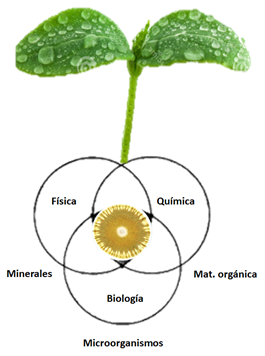
\includegraphics[width=0.4\textwidth]{images/1.png}
   \caption{\textit{Cromatografía interrelaciona la parte física, química y biológica del suelo.}}
   \end{figure}	

En base a estos tres factores mencionados en la Figura 1, la calidad del suelo se compone de tres elementos esenciales para un adecuado funcionamiento (las 3M): los microorganismos, los minerales y la materia orgánica.

\begin{figure}[H]
 \centering	
   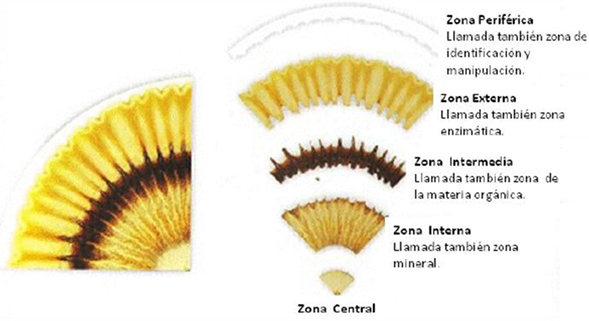
\includegraphics[width=0.7\textwidth]{images/2.png}
   \caption{\textit{Zonas de una cromatograma.}}
   \end{figure}	